% appendix_a.tex

\chapter{Zusätzliche Daten und Informationen}
\label{appendix_a}

\section{Erstellung eines flexiblen Interfaces mit FastAPI und Swagger}

Mit \texttt{FastAPI} und \texttt{Swagger} lässt sich ein flexibles und interaktives API-Interface für das 
Framework erstellen, das eine umfassende Dokumentation sowie effiziente Testmöglichkeiten bereitstellt.
Siehe Abbilung \ref{fig:Swagger_UI} für eine Darstellung der \textit{Swagger UI}.

\section{Benutzerfreundliche Interface, um das Framework zu testen}

Beispiel für eine benutzerfreundliche Oberfläche, um das Framework zu testen und die API-Endpunkte zu überprüfen.

\section{Vergleich von Optimierungstechniken für ML-Modelle}

In Tabelle \ref{tab:appendix_table} wird ein Vergleich verschiedener Optimierungstechniken für Machine-Learning-Modelle.

\section{Interviewleitfaden}

Ein Interviewleitfaden zur Anforderungsanalyse für das Framework ist in Anhang \ref{appendix:interviewleitfaden} zu finden.

\begin{figure}[h!]
    \centering
    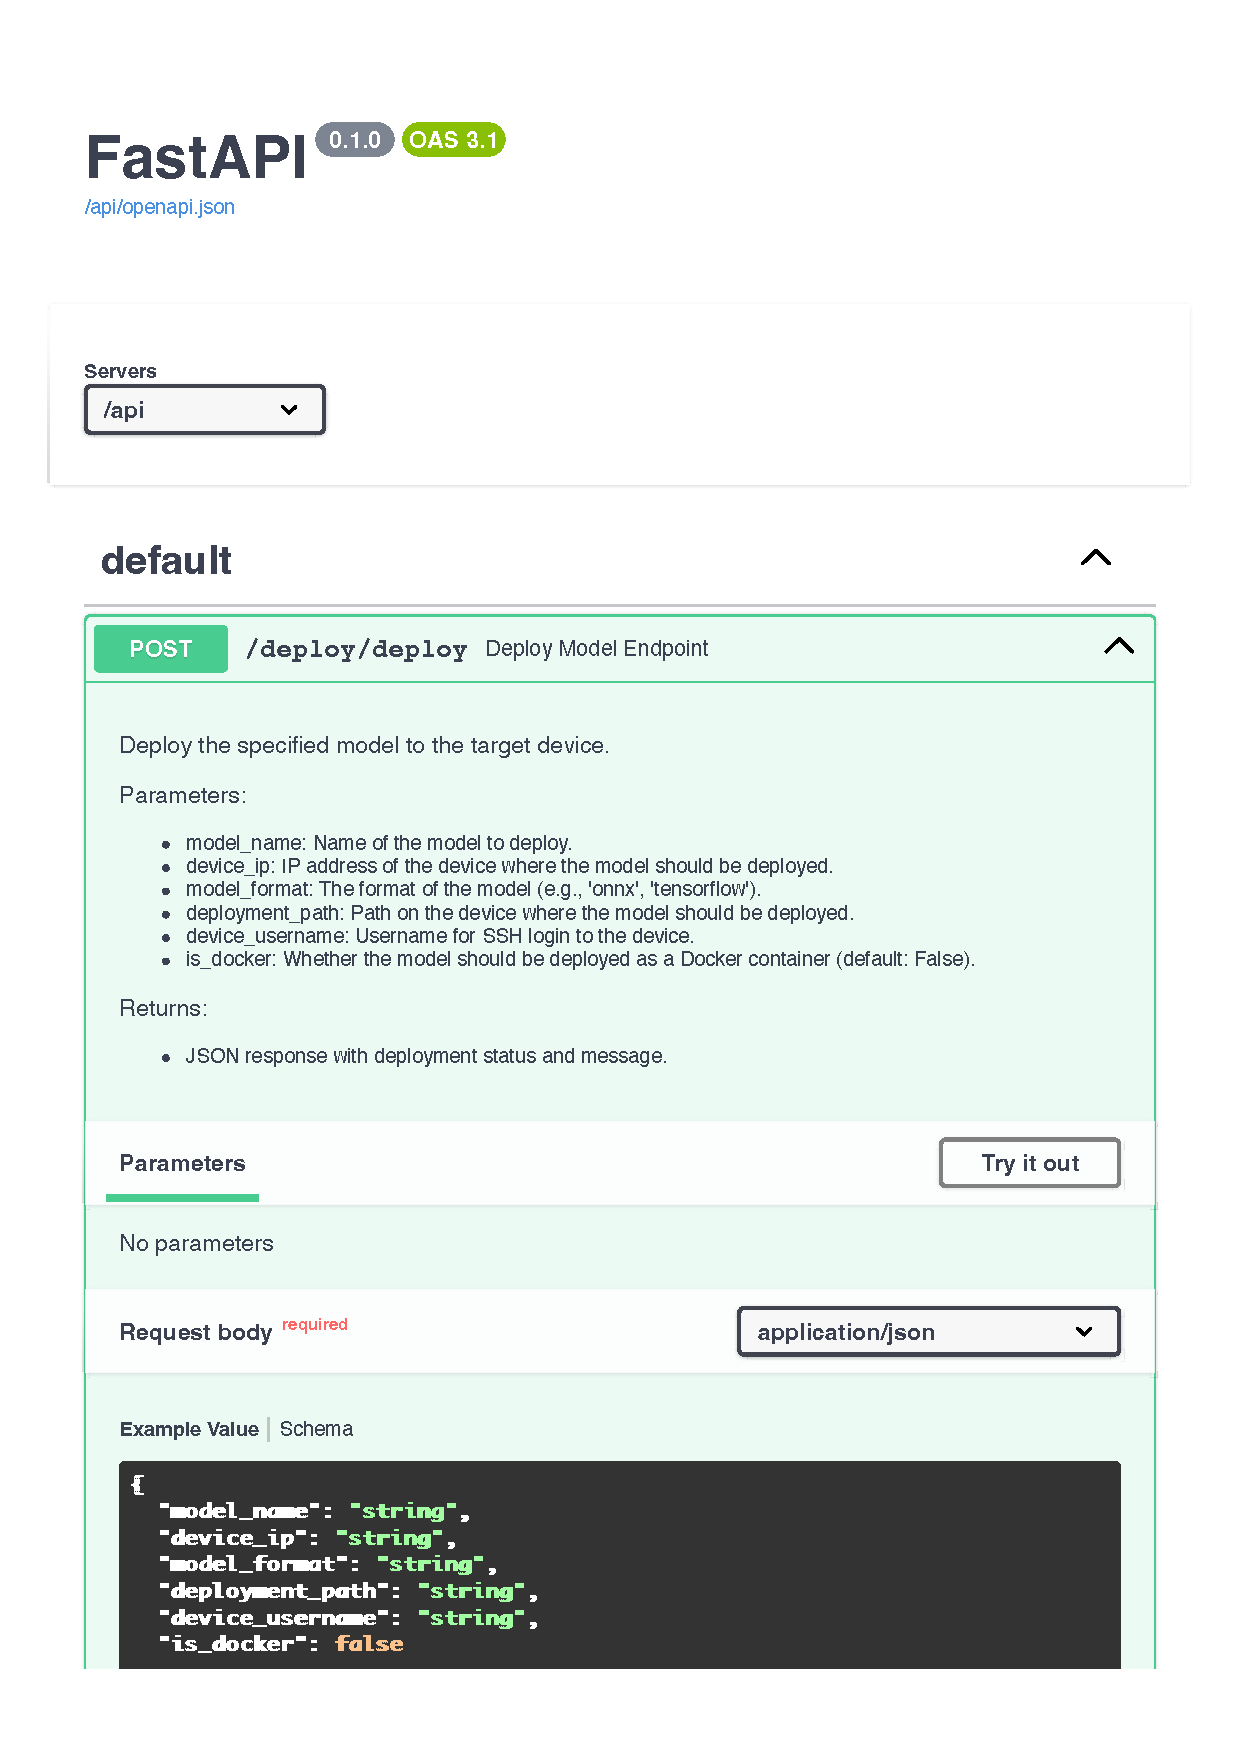
\includegraphics[width=1\textwidth]{FastAPI_Swagger_UI.pdf} 
    \caption{Framework-API mit Swagger UI} 
    \label{fig:Swagger_UI} 
\end{figure}


\begin{sidewaystable}[h!]
    \centering
    \caption{Vergleich von Optimierungstechniken für ML-Modelle}
    \begin{tabular}{|l|p{4cm}|p{4cm}|p{4cm}|p{4cm}|}
    \hline
    \textbf{Optimierungstechnik} & \textbf{Modellgröße} & \textbf{Effizienz (Latenz/Durchsatz)} & \textbf{Einfluss auf Genauigkeit} & \textbf{Anwendungsbeispiel} \\ \hline
    \textbf{Quantisierung} & Reduziert Speicherbedarf stark (durch Umwandlung in 8-Bit-Ganzzahlen) & Signifikant verbessert, besonders bei Inferenzzeiten & Geringer Einfluss bei sorgfältiger Anwendung, besonders mit Quantization-Aware Training & Mikrocontroller und Systeme mit geringer Rechenleistung \\ \hline
    \textbf{Pruning} & Reduziert Größe durch Entfernen unnötiger Verbindungen & Effizienz verbessert, aber erfordert zusätzliche Schritte im Training & Minimaler Einfluss bei unstrukturiertem Pruning; strukturiertes Pruning kann leicht die Genauigkeit senken & Tiefe neuronale Netze auf SPS und IPCs \\ \hline
    \textbf{Modellkompression} & Sehr effektive Reduktion redundanter Parameter, besonders bei großen Modellen & Effizienz gesteigert durch schnelleren Zugriff auf Speicher & Kaum signifikante Einbußen bei großen, komplexen Modellen & Edge-Devices und Systeme mit variierenden Speicheranforderungen \\ \hline
    \textbf{Knowledge Distillation} & Reduziert Größe erheblich, da komplexes Modell durch kleineres „Schülermodell“ ersetzt wird & Effizienz durch geringeren Speicherverbrauch und schnellere Berechnungen erhöht & Kann zu leichtem Genauigkeitsverlust führen; abhängig von der Distillation-Methode & Mobile Geräte und Echtzeitsysteme \\ \hline
    \textbf{Weight Clustering} & Mittlere Reduktion, da gleiche Gewichte gruppiert und komprimiert werden & Geringfügige Effizienzverbesserung & Bei grober Clusterung kann die Genauigkeit leiden & Geringfügig ressourcenbeschränkte Systeme \\ \hline
    \end{tabular}
    \label{tab:appendix_table}
\end{sidewaystable}

\begin{figure}[h!]
    \centering
    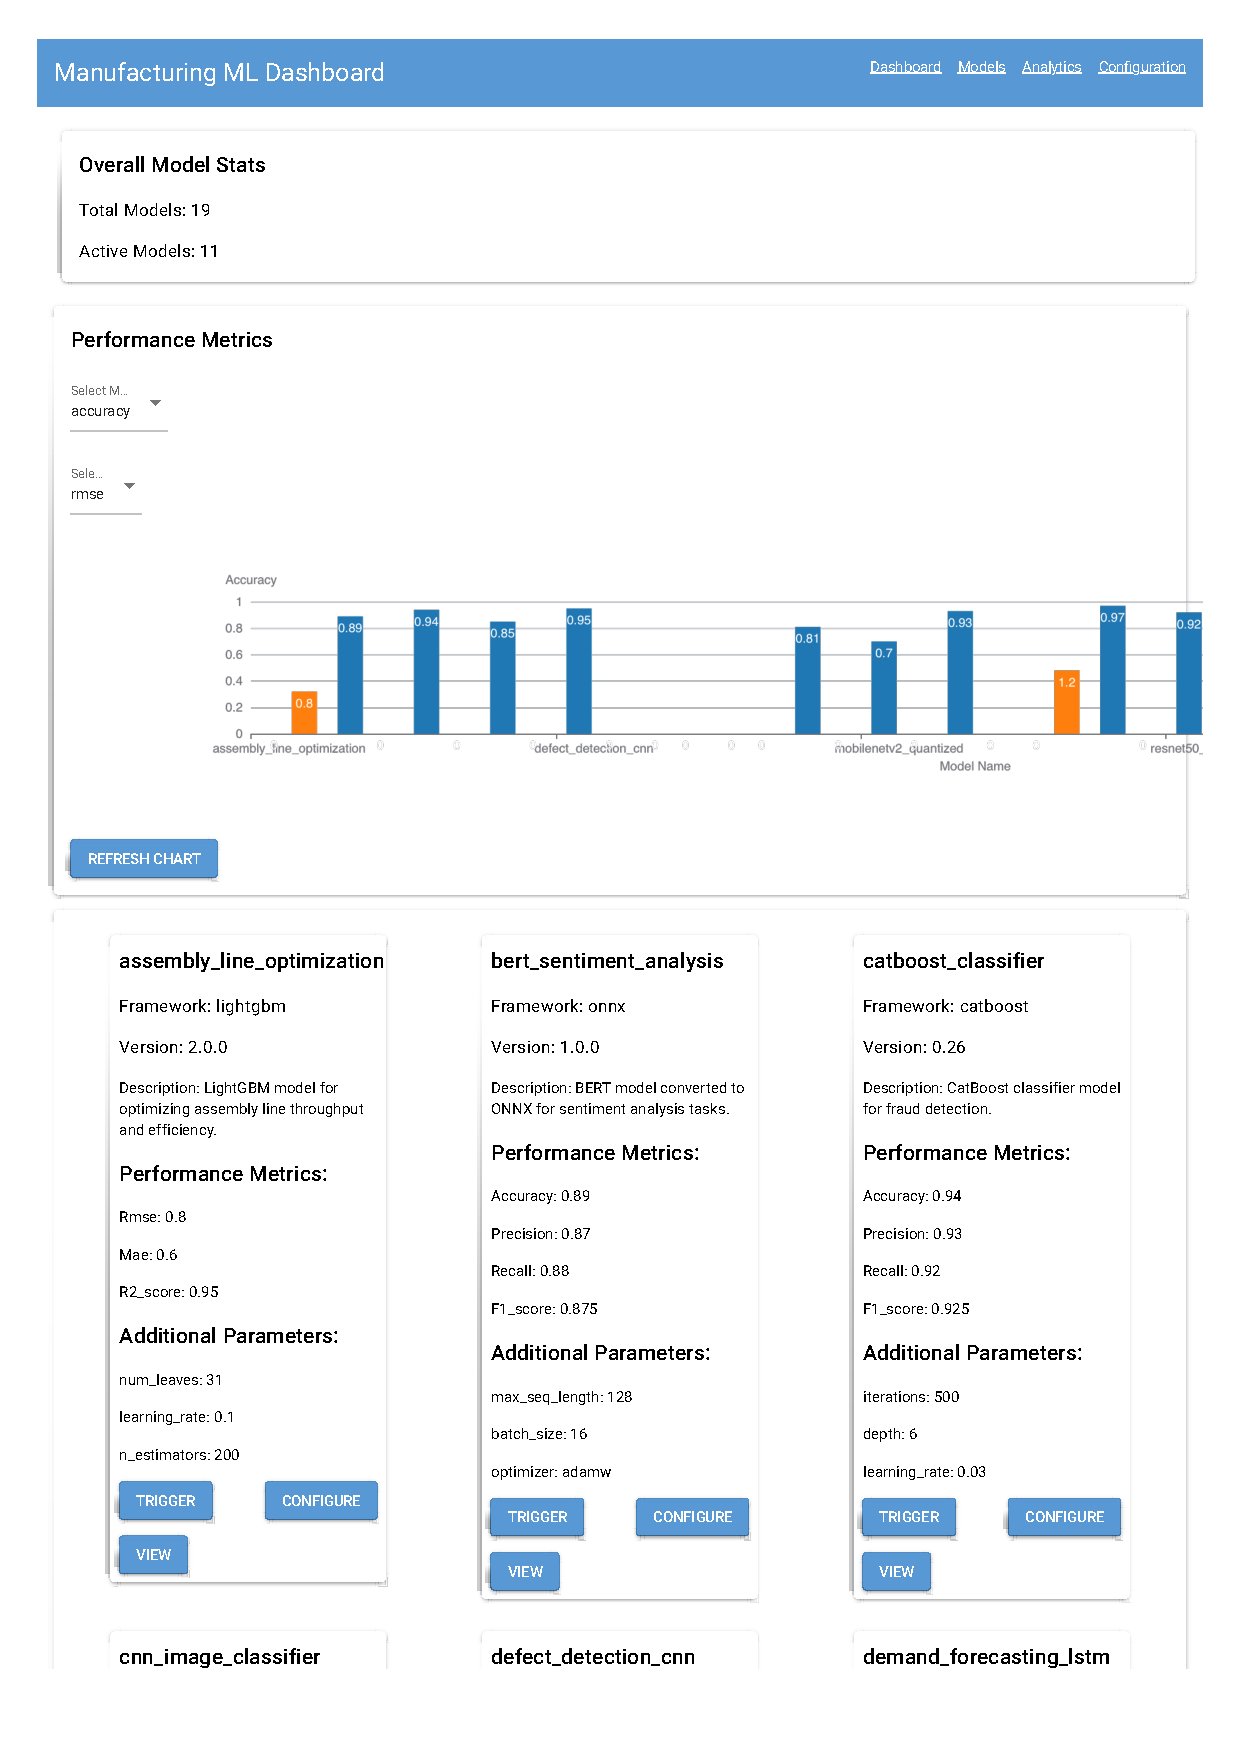
\includegraphics[width=1\textwidth]{NiceGuiModelsInformation.pdf} 
    \caption{Übersicht über verfügbare ML-Modelle} 
    \label{fig:NiceGUI_Models}
\end{figure}

\chapter{Interviewleitfaden zur Anforderungsanalyse}
\label{appendix:interviewleitfaden}

\section*{Ziel des Interviews}
\begin{itemize}
    \item \textbf{Ziel}: Identifikation spezifischer Anforderungen und Herausforderungen für die Implementierung eines Machine-Learning-Frameworks auf Embedded Systems in industriellen Umgebungen.
    \item \textbf{Teilnehmer}: Industriepartner, technische Experten, potenzielle Nutzer des Frameworks
    \item \textbf{Dauer}: ca. 45–60 Minuten
\end{itemize}

\section*{Abschnitt 1: Einführung und Kontext}
\begin{enumerate}
    \item \textbf{Vorstellung und Einführung}: Kurzvorstellung der Teilnehmer und Erläuterung des Ziels des Interviews.
    \begin{itemize}
        \item „Könnten Sie sich bitte kurz vorstellen und beschreiben, welche Rolle Sie in Ihrem Unternehmen haben?“
        \item „Wir arbeiten an der Entwicklung eines ML-Frameworks für Embedded Systems. Dieses Interview hilft uns, Ihre spezifischen Anforderungen und Herausforderungen zu verstehen.“
    \end{itemize}
    \item \textbf{Erläuterung des Projektziels}: Erklärung, warum das Feedback des Teilnehmers wichtig ist.
    \begin{itemize}
        \item „Unser Ziel ist es, das Framework so zu gestalten, dass es optimal in industrielle Umgebungen integriert werden kann. Dazu möchten wir Ihre praktischen Erfahrungen und Anforderungen besser verstehen.“
    \end{itemize}
\end{enumerate}

\section*{Abschnitt 2: Technische Anforderungen und Hardware-Beschränkungen}
\begin{enumerate}
    \item \textbf{Rechenleistung}
    \begin{itemize}
        \item „Welche spezifischen Anforderungen bestehen in Bezug auf die Rechenleistung der Embedded Systems, die Sie derzeit einsetzen?“
        \item „Gibt es bestimmte Aufgaben, die besonders viel Rechenkapazität erfordern und für das ML-Framework relevant sind?“
    \end{itemize}
    \item \textbf{Speicher- und Ressourcenbegrenzungen}
    \begin{itemize}
        \item „Mit welchen Speicher- und Hardwarebeschränkungen sind Sie in Ihrer Umgebung konfrontiert?“
        \item „Sind Speicheroptimierungstechniken wie Pruning oder Quantisierung in Ihrer Anwendung notwendig?“
    \end{itemize}
\end{enumerate}

\section*{Abschnitt 3: Energieeffizienz}
\begin{enumerate}
    \item \textbf{Bedeutung des Energieverbrauchs}
    \begin{itemize}
        \item „Inwieweit ist der Energieverbrauch in Ihrem Anwendungsfall ein kritischer Faktor?“
        \item „Sind spezielle Maßnahmen erforderlich, um den Energieverbrauch zu optimieren? Falls ja, welche?“
    \end{itemize}
    \item \textbf{Akzeptable Energiebereiche}
    \begin{itemize}
        \item „Gibt es konkrete Vorgaben oder Benchmarks, an denen sich der Energieverbrauch orientieren sollte?“
    \end{itemize}
\end{enumerate}

\section*{Abschnitt 4: Echtzeitanforderungen}
\begin{enumerate}
    \item \textbf{Echtzeitfähigkeit}
    \begin{itemize}
        \item „Welche zeitlichen Anforderungen bestehen für die Verarbeitung von ML-Modellen in Ihrer Anwendung?“
        \item „In welchen Anwendungen ist die Latenzzeit besonders kritisch?“
    \end{itemize}
    \item \textbf{Durchsatz und Datenverarbeitungsgeschwindigkeit}
    \begin{itemize}
        \item „Gibt es Anforderungen an die maximale Anzahl an Vorhersagen pro Sekunde, die das System verarbeiten muss?“
        \item „Inwiefern ist die Konsistenz der Vorhersagezeiten für Sie von Bedeutung?“
    \end{itemize}
\end{enumerate}

\section*{Abschnitt 5: Flexibilität und Erweiterbarkeit}
\begin{enumerate}
    \item \textbf{Modellflexibilität}
    \begin{itemize}
        \item „Wie wichtig ist Ihnen die Möglichkeit, das ML-Modell im laufenden Betrieb zu aktualisieren oder zu erweitern?“
        \item „Inwiefern spielt die Modularität des Frameworks für zukünftige Anpassungen eine Rolle?“
    \end{itemize}
    \item \textbf{Erweiterbarkeit und Kompatibilität}
    \begin{itemize}
        \item „Gibt es spezifische Anforderungen an die Kompatibilität mit bestehenden Systemen oder an mögliche zukünftige Erweiterungen?“
    \end{itemize}
\end{enumerate}

\section*{Abschnitt 6: Integration und Betrieb}
\begin{enumerate}
    \item \textbf{Integration in bestehende Systeme}
    \begin{itemize}
        \item „Welche Herausforderungen sehen Sie bei der Integration des Frameworks in Ihre bestehende Infrastruktur?“
        \item „Sind bestimmte Kommunikationsprotokolle oder Schnittstellen erforderlich?“
    \end{itemize}
    \item \textbf{Deployment und Wartung}
    \begin{itemize}
        \item „Welche Anforderungen bestehen an das Deployment und die Wartung der ML-Modelle in Ihrer Umgebung?“
        \item „Ist ein automatisiertes Deployment- und Aktualisierungssystem für Sie relevant?“
    \end{itemize}
\end{enumerate}

\section*{Abschnitt 7: Abschluss und Zusammenfassung}
\begin{enumerate}
    \item \textbf{Zusammenfassung der Erkenntnisse}
    \begin{itemize}
        \item „Lassen Sie uns kurz die wichtigsten Punkte zusammenfassen: Was sind Ihrer Meinung nach die drei wichtigsten Anforderungen an das Framework?“
    \end{itemize}
    \item \textbf{Feedback und Abschluss}
    \begin{itemize}
        \item „Gibt es noch andere Punkte, die wir bisher nicht besprochen haben, die aber Ihrer Meinung nach für das Framework entscheidend wären?“
\end{itemize}
\end{enumerate}

\section*{Hinweise zur Durchführung des Interviews}
\begin{itemize}
    \item \textbf{Klarheit und Struktur}: Jede Frage sollte klar formuliert und zielgerichtet sein. Der Leitfaden ist nach Themen gegliedert, um den Ablauf zu erleichtern und nichts Wichtiges auszulassen.
    \item \textbf{Flexibilität}: Der Leitfaden dient als Orientierung und kann flexibel angepasst werden, falls während des Interviews interessante neue Aspekte aufkommen.
 \end{itemize}
